\documentclass[]{article}
\usepackage{tikz}
\usepackage{pgf}
\usetikzlibrary{mindmap}
\usepackage[left=1cm,right=1cm]{geometry}
\pagestyle{empty}
\begin{document}

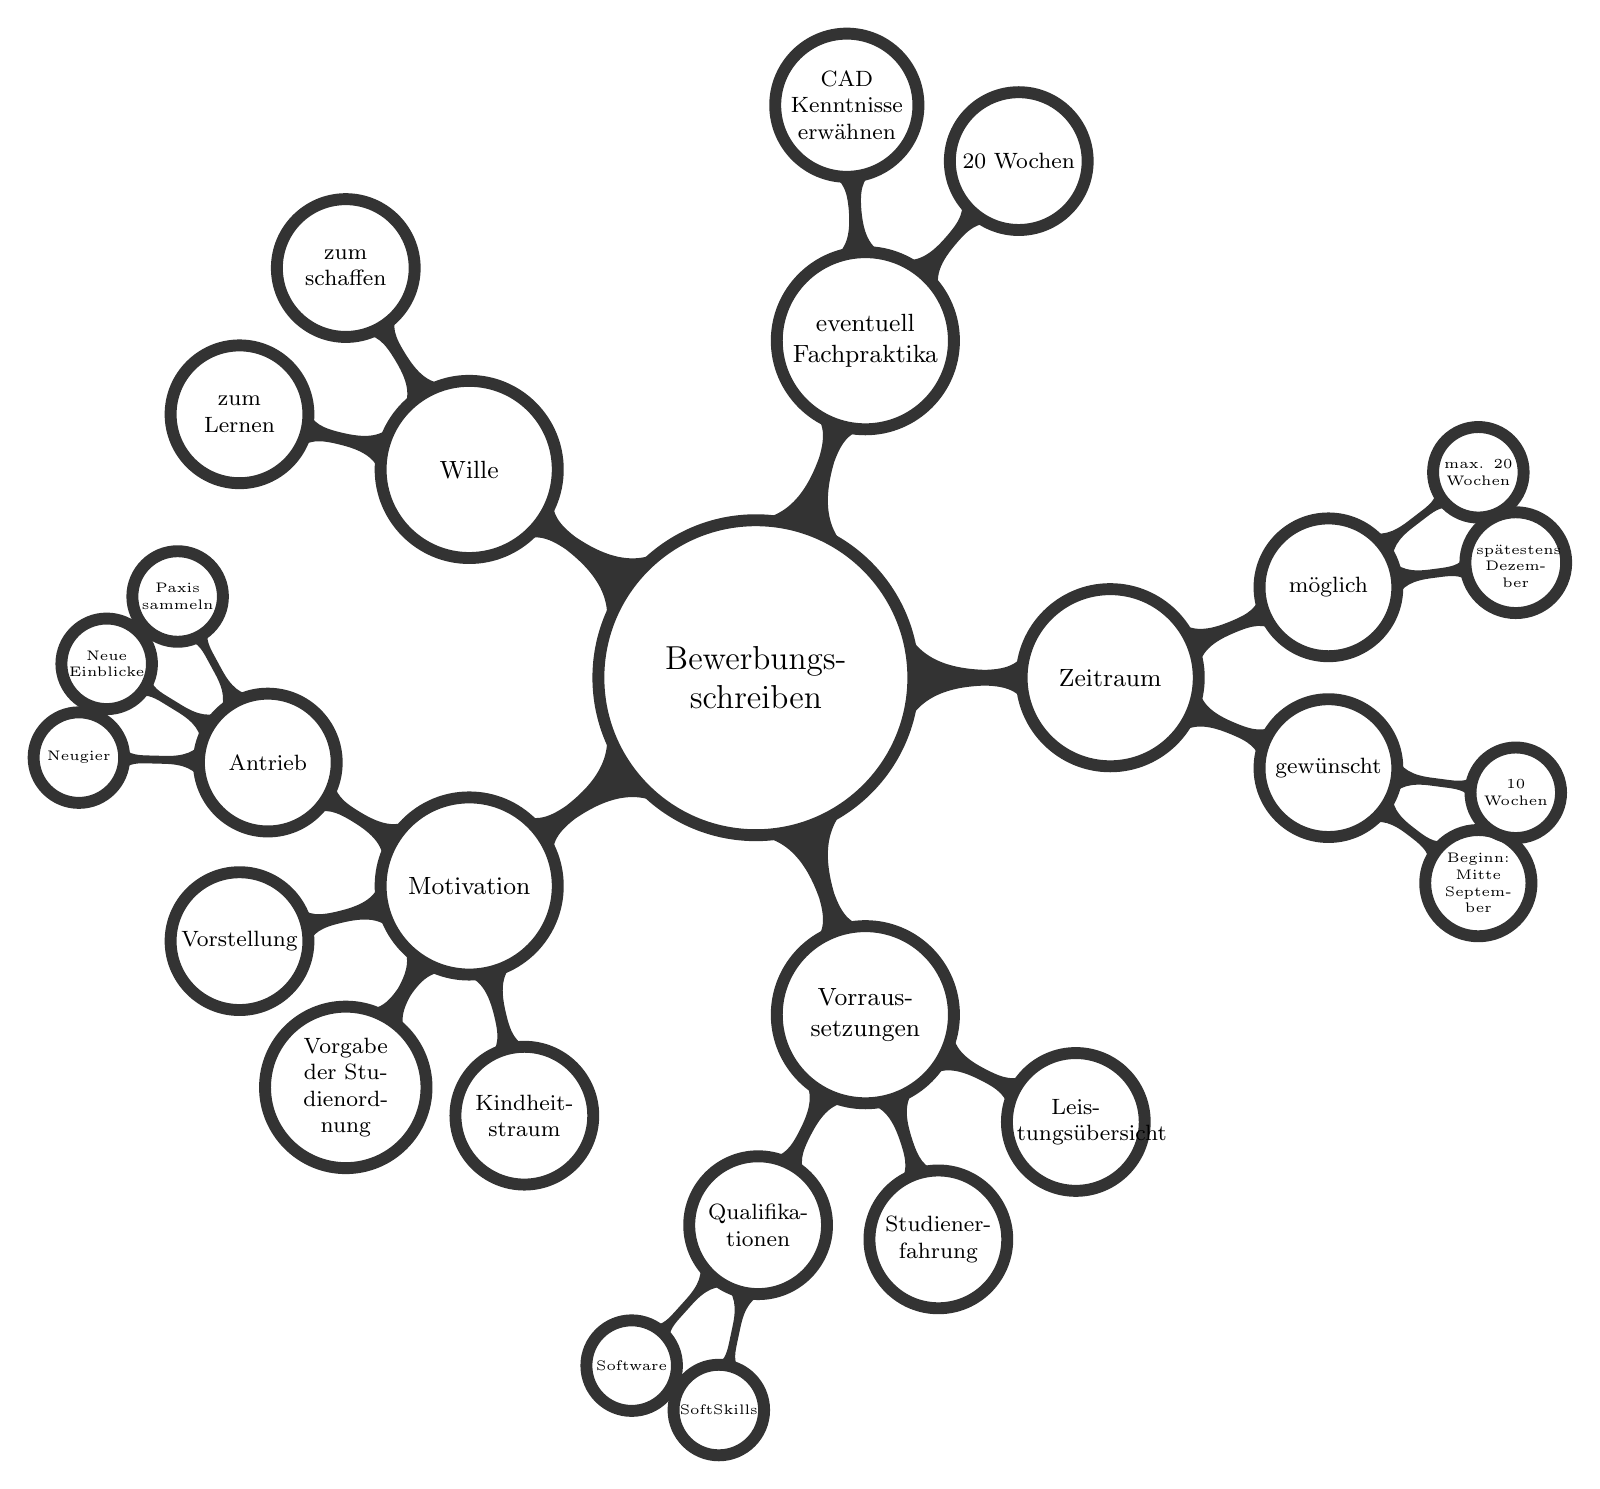
\begin{tikzpicture}	[mindmap,
every node/.style={concept, execute at begin node=\hskip0pt , fill=white, line width=1ex, text=black},
concept color=black!80,
grow cyclic,
level 1/.append style={level distance=4.5cm,sibling angle=72},
level 2/.append style={level distance=3cm,sibling angle=45},
level 3/.append style={line width=0.5ex, fill=red}]
		
\node[root concept]{Bewerbungs-schreiben} %root
child 	{ node {Motivation}
			child { node {Antrieb} 
							child{node{Paxis sammeln}}
							child{node{Neue Einblicke}}
							child{node{Neugier}} }
			child {node{Vorstellung}}
			child {node{Vorgabe der Studienordnung}}
			child {node{Kindheitstraum}}
		}
child 	{ node {Vorraussetzungen }
			child {node{Qualifikationen} child{node{Software}} child{node{SoftSkills}}}
			child {node{Studienerfahrung}}
			child {node{Leistungsübersicht}}
		}
child 	{node{Zeitraum} 
			child{node{gewünscht}
						child {node{Beginn: Mitte September}}
						child {node{10 Wochen}} } 
			child{node{möglich} 
						child {node{spätestens Dezember}}
						child {node{max. 20 Wochen}} }
		}
child {node{eventuell Fachpraktika }
			child {node{20 Wochen}}
			child {node{CAD Kenntnisse erwähnen}} }
child {node{Wille} 
			child {node{zum schaffen}}
			child {node{zum Lernen}} }
;
\end{tikzpicture}


\end{document}